%=======================================================================
\section{Technical implementation of \texttt{molecfit}}\label{app:mf}
\textbf{COMMENT by WK:} This section is based on the approach implemented in XShooter! Needs probably to be adapted for METIS!\\[1cm]

The overall strategy for the telluric correction incorporated in the METIS pipeline is outlined in Section~\ref{ssec:tellcorr}. As sort summary here: Therre are three foreseen possibilities: (a) cl
This section is intended to be a summary on how the package \texttt{molecfit} will be used for the \ac{METIS} pipeline. As it will be incorporated in the \ac{IFU} and both \ac{LSS} modes in the same way, we describe here the technical implementation only once for all pipelines. The overall strategy is described in Section~\ref{ssec:tellcorr}, more details on the \mf algorithm can be found in \cite{molecfit} and references therein.
\begin{figure}[ht]
  \centering
  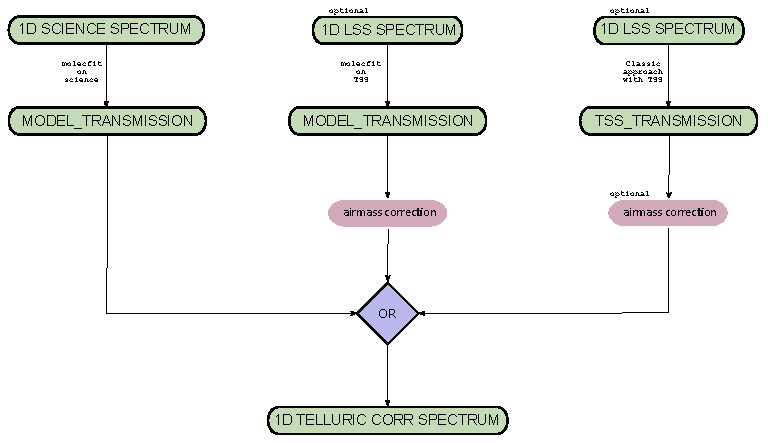
\includegraphics[width=0.9\textwidth]{figures/tell_corr_methods.pdf}
    \caption[Methods for the telluric correction to be included in the METIS pipeline]{%
        Methods for the telluric correction to be included in the \ac{METIS} pipeline.}
  \label{Fig:tellcorrmethods}
\end{figure}

%=======================================================================
\subsection{Principles}\label{app:mf_principles}
The software \texttt{molecfit} is provided by \ac{ESO} via the \texttt{telluriccorr} package. It incorporates three individual recipes: \texttt{XXX\_mf\_model}, \texttt{XXX\_mf\_calctrans}, and \texttt{XXX\_mf\_correct} (being \texttt{XXX} the prefix of the respective pipelines, e.g. \texttt{met\_lm\_lss}). The first recipe aims at fitting telluric features visible in the spectra with the help of a radiative transfer code, a line database and an atmospheric profile. This best fit is done on small wavelength regions only, where specific features of atmospheric molecules are visible. Having this best fit at hand, the transmission curve is calculated on the whole wavelength regime of the input spectrum (recipe \texttt{XXX\_mf\_calctrans}). The final telluric correction is performed by the last recipe \texttt{XXX\_mf\_correct}. For more details on the actual algorithms in \texttt{molecfit} we refer the user to the respective User Manual \cite{molecfit}.\\

%=======================================================================
\subsection{Input}\label{app:mf_input}
All three recipes require the usual \texttt{sof} file and a \texttt{.rc} file with parameters as input.
\subsubsection{\texttt{XXX\_mf\_model}}
Following the User Manual of \mf\cite{molecfit} the first recipe requires a 1d-spectrum as input, either a science observation or a telluric standard star. This means that from both, \ac{IFU}-cubes and 2d-\ac{LSS}-data one-dimensional spectra need to be extracted beforehand. For the time being we assume that the best-fit model done on that 1d-spectrum is sufficient to correct the entire \ac{IFU} cube. If it turns out that one of the fitting parameters shows major variations over the \ac{FoV} (especially the the \ac{LSF}), best-fit models need to be created for each spaxel. For the \ac{LSS} spectra we do not assume large \ac{LSF} variations along the slit. \\
%---------------------------------------------------------------------
\paragraph{\texttt{sof}-files\newline}\label{app:mf_model_sof}
The required input files for the recipe is listed in Tab.~\ref{tab:sof_mf_model}. Note that for the mandatory 1d-input spectra only one out of them is expected.
\begin{landscape}
\begin{table}[h!]
\centering
\begin{tabular}{|c : r : c : c : c|} 
 \hline
 observing  & input & \texttt{sof}-tag & mandatory$^a$ / & expected \\ 
 mode       & type & \FITS{PRO.CATG}  & optional    & number\\ 
 \hline
 LM LSS & science spectrum & \PROD{LM_LSS_SCI_1D} & mandatory & 1 \\ 
  & science spectrum (flux cal.) & \PROD{LM_LSS_SCI_FLUX_1D} & mandatory & 1 \\ 
  & telluric spectrum & \PROD{LM_LSS_STD_1D} & mandatory & 1 \\ 
 \hdashline
 N LSS & science spectrum & \PROD{N_LSS_SCI_1D} & mandatory & 1 \\ 
 & science spectrum (flux cal.) & \PROD{N_LSS_SCI_FLUX_1D} & mandatory & 1 \\ 
  & telluric spectrum & \PROD{N_LSS_STD_1D} & mandatory & 1 \\ 
 \hdashline
 LM IFU & extracted 1d science spectrum & TBD & mandatory & 1 \\ 
  & extracted 1d science spectrum (flux cal.) & TBD & mandatory & 1 \\ 
 \hline
 ALL modes & Atmospheric profile & TBD & optional & 1 \\ 
           & GDAS profile & TBD & optional & 1 \\ 
           & KERNEL library & TBD & optional & 1 \\ 
           & inclusion regions & TBD & optional & 1 \\ 
           & exclusion regions & TBD & optional & 1 \\ 
           & pixel excl. list & TBD & optional & 1 \\ 
           & list of molecules & TBD & optional & 1 \\ 
\hline
\end{tabular}
\caption{Expected content of the \texttt{sof}-file for the recipe \texttt{XXX\_mf\_model}\label{tab:sof_mf_model}.
\newline $^a$Note that from the mandatory input spectra only one out of them is needed, i.e. choose one of the \texttt{sof}-tags.}
\label{table:1}
\end{table}
\end{landscape}
%---------------------------------------------------------------------
\paragraph{\texttt{rc}-files\\}\label{app:mf_model_rc}
Due to the complexity of \mf a large set of parameters are required. As it is beyond the scope of this document to list all of them, we refer to App.~B in \cite{molecfit}. From the technical point-of-view, these parameters should have decent default values (which are to be determined), but changeable by the user, and then passed over to \mf via the recipe. 

